\chapter{Governance thresholds}\label{ch:thresholds}

Many people who work on release decisions believe that the threshold is already
set, either by the law or by a rule the institution has applied for years. The
belief has a strong form. A central bank in the European System of Central Banks
works under a precise legal duty of statistical confidentiality, written into
Council Regulation (EC) No 2533/98 \citep{ec2533,ec951}. Where natural persons are
concerned, data protection law adds its own test \citep{gdpr2016}. Statistical
offices have published threshold rules for decades, such as withholding a cell
unless it holds a minimum number of units or contributors, and these rules are
described in the standard handbook \citep[ch.~4]{hundepool2012}. On this view a
committee has no tolerance to choose. It applies the law through the rule, and the
rule is the threshold.

Two facts break the belief. The first is that the law gives no number. Recital 26
of the General Data Protection Regulation asks whether identification is
``reasonably likely'' by the means an adversary could use \citep{gdpr2016}, and
the confidentiality duty of the European System of Central Banks forbids disclosure
without saying what probability of identification counts as disclosure. The second
is that a minimum cell count does not fix a risk. On the synthetic credit register
of this book, at one tolerance of 0.12, the floor that meets the tolerance is 1 for
an adversary who holds one release, 75 for one who pools six monthly vintages and
knows when the target's loan was live, and 150 for one who also reads the loan's
exposure in each vintage. Against an insider who knows exposure closely, no floor up
to 300 meets it.
% source: paper/bis_ifc_full.tex, abstract (line 59) and Table tab:robust (paper/generated/table_robustness.tex); paper/generated/table_tolerance_floors.tex
A floor of five, applied as a rule, meets the tolerance against the first adversary
and fails against the other three. The rule is the same in each case. What changed
is the attack, and the rule does not say which attack it was written for.

The pattern is older than this book. \citet{sweeney2000} found that date of birth,
sex and postcode identify most of the population of the United States. Files that
had been stripped of names, as the conventions of the time required, could still
be linked to people through those three fields. The convention described a
procedure. It did not state a risk, so nobody could check whether the procedure
delivered one.

At the Bank, the question arrived as a request. Tom\'as, a visiting researcher,
asked for three products drawn from the credit register: the published quarterly
aggregates, a loan-level research extract for six months, and the same extract
again after a revision. The chair asked Naledi what the Bank's rule said. The
Bank's rule was a minimum of five loans in every published cell. Naledi's answer was
that the rule said how the file would be protected, and that nothing in it said how
much risk the Bank would accept, against whom, or on whose authority.

This chapter answers one question. What must a release threshold contain before it
can decide anything, and who must write each part of it?

\section{What the law asks and what it leaves open}\label{c07:sec-law}

The legal basis of a release is the source of the duty and the list of those it
protects. For the national central banks of the European System of Central Banks,
the duty to keep statistical information confidential comes from Article 8 of
Council Regulation (EC) No 2533/98, as amended by Council Regulation (EC) No
951/2009 \citep{ec2533,ec951}. For European statistics produced by national
statistical authorities, it comes from Regulation (EC) No 223/2009 \citep{ec223}.
Where natural persons are concerned, the General Data Protection Regulation applies
to data that relate to an identifiable person, and Recital 26 says that account
should be taken of all the means ``reasonably likely'' to be used to identify the
person, directly or indirectly \citep{gdpr2016}.

None of these texts gives a probability. They could not sensibly do so, because
the probability of identification depends on who holds the release, what else they
hold, and what they stand to gain, and these differ from one product to the next.
The law sets the duty and leaves the reading of it to the institution. A tolerance
is the institution's written reading of ``reasonably likely'' for a declared
adversary and a declared harm, and the record should say that this is what it is.
A reading can be disputed, revised and defended; a reading that was never written
down can only be inferred after the event, usually by someone hostile to the
institution.

The law also fixes whom the duty protects, and for a credit register the answer has
three parts. The borrowers are protected: firms whose loans, exposures and arrears
the register holds. The reporting agents are protected: the lenders whose positions
and customer relationships the register records, and whose contributions another
lender might reconstruct from published totals. And the natural persons behind
some borrowers are protected, such as sole traders, for whom a firm's credit record
is a personal record and data protection law applies. The three need not share one
tolerance. A lender's position reconstructed by a competitor is a commercial harm;
a sole trader's arrears made public is a personal one. A tolerance that names its
protected parties can be set at the level each warrants, and one that does not will
be set, without anyone deciding so, at the level of whichever party the analyst had
in mind.

\section{Assembling the legal element}\label{c07:sec-legal-assembly}

The legal element is the one the code cannot check, so it is written out. Record, in order: the harm class the law recognises; the protected parties; the access route by which the data reach an adversary; the argument that the attack is reasonably likely, with the evidence for each term; the horizon over which the statement holds; and the event that triggers a revisit. These are the fields the strict check lists when they are empty. The book gives no legal advice, and counsel fills these fields.

\section{The nine elements of a threshold}\label{c07:sec-elements}

A governance threshold, in the sense of this book, is a tolerance together with the
things that turn a number into a decision.

\begin{definition}[Governance threshold]\label{c07:def-thresh}
A governance threshold is the tuple
\begin{equation}\label{c07:eq-tuple}
G = (\tau,\ o,\ d,\ a,\ h,\ \alpha,\ \ell,\ s,\ m),
\end{equation}
where $\tau \in (0,1)$ is the risk tolerance; $o$ is the named owner who accepts
the residual risk; $d$ is the expiry date; $a$ is the adversary specification; $h$
is the harm class to which the tolerance applies; $\alpha$ is the accepted
probability of a wrong release; $\ell$ is the legal basis together with the parties
it protects; $s$ is the access route; and $m$ is the horizon, the number of releases
or vintages over which a programme's pooled risk is assessed. For a threshold that
governs one release only, $m = 1$.
\end{definition}

Figure~\ref{c07:fig-elements} arranges the nine elements by the question each
answers. Five fix what the number refers to: the adversary, the harm class, the
protected parties and legal basis, the access route and the horizon. Two fix how
much risk is accepted and how sure the institution must be: the tolerance and the
error probability. Two fix who answers for the decision and until when: the owner
and the expiry. A risk table, however careful, supplies none of the nine. It
supplies the evidence against which they are applied.

\begin{figure}[ht]
\centering
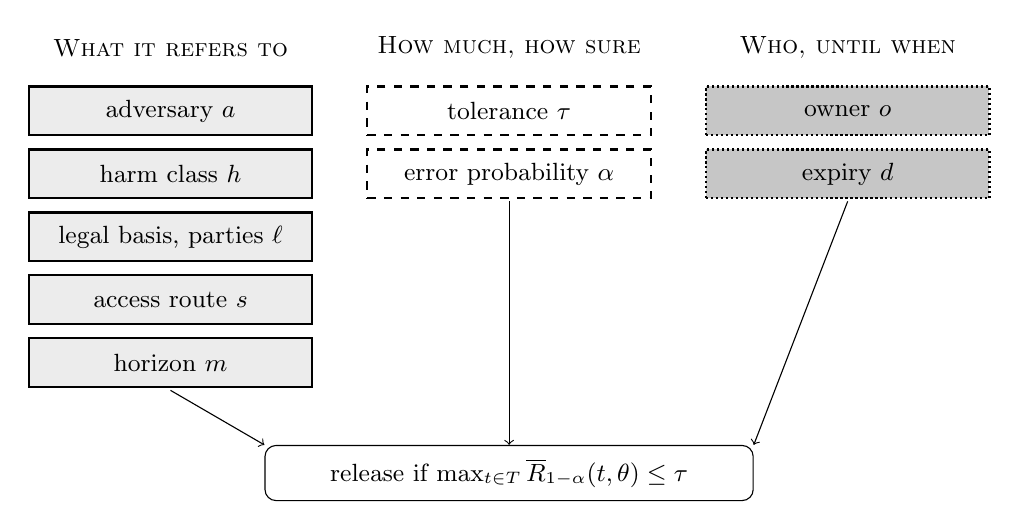
\begin{tikzpicture}[x=1cm,y=1cm,
  el/.style={draw, minimum width=3.6cm, minimum height=0.62cm, font=\small, inner sep=2pt}]
\node[font=\small\scshape] at (-4.3,3.0) {What it refers to};
\node[el, fill=gray!15, thick] at (-4.3,2.2) {adversary $a$};
\node[el, fill=gray!15, thick] at (-4.3,1.4) {harm class $h$};
\node[el, fill=gray!15, thick] at (-4.3,0.6) {legal basis, parties $\ell$};
\node[el, fill=gray!15, thick] at (-4.3,-0.2) {access route $s$};
\node[el, fill=gray!15, thick] at (-4.3,-1.0) {horizon $m$};
\node[font=\small\scshape] at (0,3.0) {How much, how sure};
\node[el, fill=white, dashed, thick] at (0,2.2) {tolerance $\tau$};
\node[el, fill=white, dashed, thick] at (0,1.4) {error probability $\alpha$};
\node[font=\small\scshape] at (4.3,3.0) {Who, until when};
\node[el, fill=gray!45, densely dotted, thick] at (4.3,2.2) {owner $o$};
\node[el, fill=gray!45, densely dotted, thick] at (4.3,1.4) {expiry $d$};
\node[draw, rounded corners, font=\small, minimum width=6.2cm, minimum height=0.7cm]
  (rule) at (0,-2.4) {release if $\max_{t \in T} \overline{R}_{1-\alpha}(t,\theta) \le \tau$};
\draw[->] (-4.3,-1.35) -- (rule.north west);
\draw[->] (0,1.05) -- (rule.north);
\draw[->] (4.3,1.05) -- (rule.north east);
\end{tikzpicture}
\caption{The nine elements of a governance threshold, grouped by the question each
answers. Light boxes with solid borders fix what the risk figure refers to; white
boxes with dashed borders fix how much risk is accepted and with what error; dark
boxes with dotted borders fix who answers for the decision and until when. All
nine feed the admissibility rule \eqref{c07:eq-admiss}.}
\label{c07:fig-elements}
\end{figure}

Each element prevents a failure that can be named. Without an owner the tolerance
belongs to nobody, and nobody has the authority to revise it. Without an expiry
date an assessment made on a register as it stood years ago governs a release
today, after the population, the products and the adversaries have all moved.
Without an adversary the number has no referent, since Chapter~\ref{ch:scenario}
showed that risk is defined only given an attack. Without a harm class a tolerance
calibrated for commercial nuisance is applied where the consequence falls on a
person. Without an error probability the institution has not said how much
evidence it requires, and Chapter~\ref{ch:estimate} showed that a rule based on a
point estimate releases about half the time at the boundary. Without the legal
basis and protected parties the tolerance has no source of duty and no list of whom
it serves. Without an access route the same tolerance is applied to products that
face different adversaries. Without a horizon a programme tolerance has no fixed
meaning, because Chapter~\ref{ch:programmes} showed that pooled risk does not fall
as releases are added, and a monthly series has no natural end.

Given the nine elements, the decision rule is short. Let
$\overline{R}_{1-\alpha}(t,\theta)$ be an upper confidence bound at level
$1-\alpha$ on the risk to target $t$ under protection setting $\theta$, with its
interpretation recorded. A release is admissible only if
\begin{equation}\label{c07:eq-admiss}
\max_{t \in T} \overline{R}_{1-\alpha}(t,\theta) \le \tau ,
\end{equation}
the assessment date precedes $d$, and the release, its users and its route fall
within the scope of $a$, $h$, $\ell$, $s$ and $m$. The rule needs one more
declaration, the target set $T$, and the next section shows why it cannot be left
implicit.

When Tom\'as's request reached the committee, Naledi brought a single page with the
nine elements as headings and blank spaces beneath them. She filled in the
adversary, the harm class and the access route herself, because the analysis
depended on them, and left the tolerance, the owner and the expiry blank. Those
were not hers to fill.

\section{Target sets and joint decisions}\label{c07:sec-targets}

The maximum in \eqref{c07:eq-admiss} runs over a set $T$, and the choice of $T$ is
part of the threshold. A maximum over every record in the file, a maximum over the
records of a protected subgroup, and an average over a declared population are
three different controls. A release can pass one while failing another, and a
committee that is told only that the release ``passed'' does not know which control
it met.

The credit register shows the difference. Large firms are few, and in a release
keyed on sector, region and size class they sit in thin cells. A uniform draw of
targets holds only a few hundred of them, so an average over all loans says little
about large borrowers. When the institution requires every firm size class to meet
the tolerance of 0.12, the floor for an adversary who holds one release rises from 1
to 20, and the floor for one who pools the vintages and knows the loan's history
rises from 75 to 200.
% source: paper/bis_ifc_full.tex, abstract (line 59): "a floor of 20 when every firm size class must pass", "75 (200 for every size class)"
For the adversary who also reads exposure in each vintage, no floor up to 200
protects every size class. The protected parties of Section~\ref{c07:sec-law} are
the natural way to choose $T$: each party, or each subgroup the institution has a
reason to protect, becomes a member of a declared family.

Requiring every subgroup to pass looks as if it should cost something in error
control, since the institution now makes several statistical claims at once. It does
not, and the reason is worth stating precisely, because the opposite intuition
leads institutions to divide $\alpha$ among subgroups and so to demand far more
evidence than the decision needs.

\begin{proposition}[Joint release over subgroups]\label{c07:prop-iut}
Let $T = \{1,\dots,G\}$ be a set of subgroups fixed before any outcome is seen, with
true risks $r_1,\dots,r_G$, and let $\overline{R}_g$ be a one-sided upper bound for
subgroup $g$ satisfying $\Prob(\overline{R}_g < r_g) \le \alpha$. Release if and only
if $\overline{R}_g \le \tau$ for every $g$. Then the probability of releasing when
some subgroup has $r_g > \tau$ is at most $\alpha$, whatever the dependence between
the bounds.
\end{proposition}

This is the intersection--union test of \citet{berger1982}. The hypothesis to be
rejected is a union, that some subgroup is unsafe, and the release requires every
subgroup's bound to reject its own part of it. A wrong release needs at least one
unsafe subgroup to pass, and the probability of that is at most $\alpha$ for that
subgroup alone. So each subgroup's bound may be taken at level $\alpha$, with no
correction for the number of subgroups. A Bonferroni correction is needed for a
different claim: to report every subgroup's bound as one simultaneous statement, or
to say that the worst subgroup lies above some value. Those are claims about the
evidence. The release decision is a claim about the release, and it needs no
correction.

The same logic covers several declared adversaries at one setting, which is how the
release chain of Chapter~\ref{ch:monitoring} tests three attacks at each floor at
the full level. It does not cover the choice of adversary after the results are
read. A committee that sees the floors each adversary requires and then declares
the adversary whose floor it prefers has chosen a hypothesis with the data. The
journal article measured the price of making that choice honest: one audit chain per
adversary at $\alpha/3$ spent a median of 13,764 attacks on the credit register,
against 6,422 for one chain that tests all three adversaries declared in advance.
% source: paper/publication_versions/table_chain_audit.tex
The cheaper route requires the adversary to be part of the threshold, written down
before the audit.

\section{Declaring the adversary}\label{c07:sec-adversary}

The adversary specification says who attacks, what it knows, which targets it
attacks, and when it acts. The last part is usually left to a convention: an
attack is counted as a success when the adversary's best guess is right, or when
its posterior probability on the guess exceeds one half. An adversary need not
follow either convention. It acts when acting pays.

Suppose a correct allegation brings the adversary a benefit $h > 0$, a false
allegation costs it $c_f \ge 0$, and making any allegation costs $c_a \ge 0$. At
posterior probability $p$ that its candidate is the target, acting has expected
payoff $ph - (1-p)c_f - c_a$.

\begin{proposition}[Economically rational attack threshold]\label{c07:prop-attack}
An adversary that maximises expected payoff, and acts when acting has nonnegative
expected payoff, never acts if $c_a \ge h$. If $c_a < h$ it acts if and only if
\begin{equation}\label{c07:eq-attack}
p \ge p^\star = \frac{c_f + c_a}{h + c_f},
\end{equation}
and then $p^\star < 1$. The threshold equals one half exactly when $h = c_f + 2c_a$.
\end{proposition}

The convention of one half is therefore one payoff structure among many: equal
stakes for right and wrong allegations, with free allegations. The repository reads
one attack on the credit register at three thresholds. An adversary that gains and
loses equally and pays nothing to allege acts at one half, acts on 0.179 of
targets, is right 0.814 of the time and collects 0.146 correct allegations per
target. An adversary that gains ten times what a false allegation costs it acts at
0.136: it acts on 0.395 of targets, is right 0.556 of the time, and collects 0.220,
half as much again. An adversary for whom a false allegation is costly, through
reputation or law, acts at 0.917, on 0.083 of targets, and is right 0.994 of the
time.
% source: paper/generated/table_adversary.tex; paper/generated/numbers.tex (\runseqequalyield, \runseqpaidthreshold, \runseqpaidcoverage, \runseqpaidprecision, \runseqpaidyield, \runseqcautiousthreshold, \runseqcautiouscoverage, \runseqcautiousprecision)

The three rows are the same attack on the same release. A journalist who would be
sued for naming the wrong firm is the third adversary. A data broker who loses
little from a wrong match and sells every right one is the second. An evaluation
that reports one threshold reports one point on a curve the adversary chooses from,
and the record should carry the curve of precision against coverage, or state the
payoffs that select the point it reports.

Pieter is the adversary the Bank's file is least able to stop. As a credit analyst
at a reporting lender he knows, closely, the exposure of every loan his own bank
has made, and he can see which months each was live. On the synthetic register an
insider who knows exposure to within one per cent and knows the history still
names 42 per cent of targets at a floor of 300.
% source: paper/publication_versions/jpc_evidence.tex, Section sec:carried ("defeats every floor up to 300, where it still names 42 per cent of targets")
No tolerance a committee could defend is met against him by suppression. Declaring
him in the threshold does not protect his bank's customers. It makes visible that
the loan-level file is the wrong product for any route Pieter can reach, which is
the subject of the next section.

\section{The access route}\label{c07:sec-route}

The same file faces different adversaries depending on how it reaches its users.
A public file can be downloaded by anyone, including those who hold the richest
auxiliary information and the strongest motive. A scientific-use file released
under contract to accredited researchers faces users who are known, bound by
agreement and limited in number. Access in a secure environment, where the
researcher works on the data inside the institution's systems and takes away only
checked outputs, removes the file from the adversary's hands altogether. These are
three routes with three threat models. The Five Safes framework treats the route as
a control in its own right, alongside safe projects, people, settings and outputs
\citep{desai2016}.

The route belongs in the threshold because it changes which adversary the
tolerance must be met against. A loan-level extract that fails as a public file,
because a pooling adversary with exposure readings needs a floor that destroys most
of it, may pass in a secure environment, where the declared adversary no longer
holds the file at all and the residual risk lies in the outputs that leave. The
assessment is then a different one: the outputs must be checked, and the users
must be accredited, and each of these has its own failure modes. What the route
does not allow is to keep the public file's assessment and change the route
afterwards, or to assess the secure route and release the public file. The
tolerance holds for the route it names.

For Tom\'as, this settled more than the analysis did. The quarterly aggregates could
be published. The loan-level extract could not be released as a file to a visiting
researcher on any floor that left it useful, because a copy holding all six
vintages would be dangerous in the hands of anyone who knew a firm's borrowing
history, as its lenders and counterparties do; it could be made available to
him in the Bank's secure environment, with outputs checked before they left. The
revised extract was a third product and would need its own record when it existed.

\section{Separating the analyst, the owner, the reviewer and audit}\label{c07:sec-roles}

The elements of a threshold are written by different people, and the separation
between them is part of what makes the threshold work. Central banks already use a
structure that fits: the three lines of defence of operational risk.

The analyst who declares the attacks and runs the simulations, and the data owner
who holds the register and knows which products are drawn from it, sit in the first
line. The analyst owns the correctness of the calculation, not the decision. The
reviewer, in a risk or methodology function outside the production line, checks
that the declared adversaries are plausible, that none was omitted for convenience,
and that the tests of the model behind the risk figure were run; this is the second
line. Internal audit is the third. It checks, after the fact, that the record was
filed, that the tolerance was signed before the first outcome was seen, and that
the controls on the audit process described in Chapter~\ref{ch:monitoring} were in
place. The owner $o$ is the senior officer who accepts the residual risk on the
institution's behalf, in a central bank typically the chair of the release
committee or the executive member responsible for statistics.

The reason for the separation is that each role has an incentive the others check.
An analyst who has seen the results can choose, in good faith, the adversary whose
floor keeps the file useful, and Section~\ref{c07:sec-targets} showed what that
choice costs. A reviewer who did not run the analysis has no stake in the floor it
produced. An owner who signs the tolerance before the analysis has no way to fit
the tolerance to the result. And an auditor who reads the record later can check
the order of events, which is the one thing the people inside the decision cannot
credibly certify about themselves. Where the institution is small and one person
must hold two roles, the analyst and the reviewer are the pair to keep apart.

Grace read the record of the decision on Tom\'as's request some months later. She
checked that the tolerance, its owner and its expiry had been signed by the chair
on a date before the first audit was registered; that the adversaries in the
record were those the reviewer had approved; that the secure-environment route was
written into the threshold and not added after the public file failed; and that
the expiry fell before the next scheduled revision of the register. She found one
gap. The record named the borrowers as protected parties and said nothing of the
lenders whose positions the extract held. The next record named them.

\section{Expiry and horizon}\label{c07:sec-expiry}

The last two elements give a threshold a life. A risk assessment describes a
register as it stood, a set of products as they were, and adversaries with the
information available to them at the time. All three change. The register gains
and loses units, new products are drawn from it, and outside sources that an
adversary can link to grow. An expiry date forces the assessment to be renewed
before its premises have drifted out of sight. It also makes the owner's acceptance
of risk bounded in time, which is easier to give and easier to defend.

The horizon does the same work across releases. Chapter~\ref{ch:programmes}
proved that no function of per-release risks bounds the risk of an adversary who
pools the releases, and that pooled risk does not decrease as releases are added. A
programme tolerance therefore needs to say over how many releases the pooled risk
was assessed. A threshold with a horizon of six monthly vintages says that the
seventh vintage needs a new assessment before it is published. One without a
horizon says nothing about the seventh, and the twelfth and the twentieth will be
published under an assessment that never considered them.

\section{The answer}\label{c07:sec-answer}

The chapter asked what a release threshold must contain before it can decide
anything, and who must write it. The law sets the duty and names the protected
parties, and it leaves the probability to the institution. A minimum cell count is
a protection setting, and it meets a tolerance only for a declared adversary. A
threshold that can decide therefore has nine elements: a tolerance and an error
probability; an adversary, a harm class, a legal basis with its protected parties,
an access route and a horizon, which fix what the tolerance refers to; and an owner
and an expiry date, which fix who answers for it and until when. The target set
must be declared with it, and a joint decision over subgroups or adversaries
declared in advance needs no division of the error probability. The analyst writes
the adversary and runs the evidence; an independent reviewer checks the adversary;
a senior owner signs the tolerance before any outcome is seen; and internal audit
checks afterwards that these things happened in that order.

\begin{inpractice}[In practice: writing a threshold]\sloppy
For each product and each harm class, write the nine elements on one page before
any risk is measured, and have the owner sign the tolerance, the error probability
and the expiry. Name the legal basis and every protected party, and set separate
tolerances where their harms differ. Declare the target set: all records, named
subgroups, or a population average. Test every declared subgroup or adversary at
the full error level, and divide the level only when reporting all the bounds as
one statement. State the payoffs the adversary is assumed to face, or report the
curve of precision against coverage. Name the access route, and reassess if the
route changes. Give a programme tolerance a horizon and set a reassessment before
the first release beyond it.

\smallskip\noindent\textit{In the software.} The threshold is
\texttt{privacy\_risk.governance.GovernanceThreshold}, and the decision is
\texttt{decide}, which returns \texttt{INVALID} when the prespecified validation
failed, \texttt{FAIL} when the assessment date falls on or after the expiry date or
when the upper bound exceeds the tolerance, and \texttt{PASS} otherwise. The class
records six of the nine elements: tolerance, owner, expiry, adversary, harm class
and error probability. It has no field for the legal basis and protected parties,
the access route or the horizon, so a record built from it must carry those three
separately, and \texttt{decide} cannot check them. \texttt{decide} also takes one
upper bound, so the maximum over the target set must be formed before it is
called. The attack threshold of Proposition~\ref{c07:prop-attack} is
\texttt{privacy\_risk.sequential.attack\_threshold}, and
\texttt{precision\_coverage} and \texttt{at\_threshold} read an attack along the
curve.
\begin{lstlisting}
@dataclass(frozen=True)
class GovernanceThreshold:
    tolerance: float
    owner: str
    expiry_date: str
    adversary: str
    harm_class: str
    alpha: float
\end{lstlisting}
\end{inpractice}

\section{Proofs}\label{c07:sec-proofs}

\begin{proof}[Proof of Proposition~\ref{c07:prop-iut}]
If no subgroup has $r_g > \tau$ there is nothing to prove. Otherwise fix one
subgroup $g^\ast$ with $r_{g^\ast} > \tau$; since the risks are fixed parameters and
$T$ was fixed in advance, $g^\ast$ does not depend on the data. A release requires
$\overline{R}_g \le \tau$ for every $g$, and in particular
$\overline{R}_{g^\ast} \le \tau < r_{g^\ast}$. Hence
\[
\Prob(\text{release}) \le \Prob(\overline{R}_{g^\ast} \le \tau)
\le \Prob(\overline{R}_{g^\ast} < r_{g^\ast}) \le \alpha .
\]
The argument uses only the marginal coverage of the one bound
$\overline{R}_{g^\ast}$, so it holds whatever the dependence between the bounds
\citep{berger1982}.
\end{proof}

\begin{proof}[Proof of Proposition~\ref{c07:prop-attack}]
At posterior probability $p$ the expected payoff of acting is
$V(p) = ph - (1-p)c_f - c_a = p(h + c_f) - (c_f + c_a)$, which is increasing in $p$
because $h + c_f > 0$. Its largest value, at $p = 1$, is $h - c_a$. If $c_a > h$,
then $V(p) < 0$ for every $p \le 1$; if $c_a = h$, then $V(p) \le 0$ with equality
only at $p = 1$, where acting gains nothing. In both cases the adversary does not
act, which we record as $p^\star = +\infty$. If $c_a < h$, then $V(p) \ge 0$ if and
only if $p \ge (c_f + c_a)/(h + c_f)$, and this ratio is below one because
$c_f + c_a < h + c_f$. Finally, $(c_f + c_a)/(h + c_f) = 1/2$ if and only if
$2c_f + 2c_a = h + c_f$, that is $h = c_f + 2c_a$.
\end{proof}
